% $Id$
% !TeX encoding = UTF-8
% !TeX spellcheck = en_US
% !TeX root = ../hdr_dfolio.tex

\Chapitre{Context of Activities}

This chapter introduces the various activities that I have conducted since as I have started being involved as researcher-teacher. 
It first starts with an overall overview of my career, that sets the background in which  my works was carried out.
This global  view contains several issues, which are synthesized, in order to explain the general structuring of my activities.Actually, as in any faculty position, my works encompass several activities, that are mainly related to teaching and research.
The organization of these tasks are then presented in \autoref{sec:activities}.
This integrates the articulations of the teaching, research, supervisions and collaboratives works in a general framework synergy.
This chapter largely refers to the appendices\;\RefCV and \RefMyRef, that include a long version of my resume, and the list of my publications respectively.


% ---------------------------------------------------------------------------------
% SECTION -------------------------------------------------------------------------
\section{Career overview}\label{sec:career}

\subsection{Doctorate degree and post-doctorate}\label{sec:career:PhD}

I have defended my \PhD in Robotics in 2007 within the  Robotics, Action, and Perception (RAP) group of the Laboratory for Analysis and Architecture of Systems\footnote{LAAS: \url{http://www.laas.fr}} (LAAS), CNRS\footnote{French National Center for Scientific Research. \url{http://www.cnrs.fr}}, under the supervision of Viviane Cadenat, Associate Professor at Paul Sabatier University of Toulouse, France. 
My \PhD thesis dealt with the design of multi-sensor based control strategies allowing a mobile robot to perform vision-based tasks amidst possibly occluding obstacles.
We have first proposed techniques able to fulfill simultaneously the mentioned objectives. 
However, avoiding both collisions and occlusions often over-strained the robotic navigation task, reducing the range of realizable missions. 
This is the reason why we have developed a second approach which lets the visual features loss occurs if it is necessary for the task realization. 
Using the link between vision and motion, we have proposed different methods (analytical and numerical) to compute the visual signal as soon it becomes unavailable. 
We have then applied them to perform vision-based tasks in cluttered environments, before highlighting their interest to deal with a camera failure during the mission.

In addition, during my doctorate degree, I also had the opportunity to perform teaching activities, first as  temporary teacher (\SI{3}{\years}), and then as teaching assistant, specifically  in French \EFrench{Attaché Temporaire d'Enseignement et de Recherche}  (ATER, \SI{1}{\year}) both for  the Paul Sabatier University of Toulouse.
These global teaching experiences have led to a total volume of \SI{308}{\hETD}\footnote{\label{foot:hETD}\glsreset{HETD}\glsdesc[hyper=false]{HETD}}.

\medskip
Between 2007 and 2008, I joined the Lagadic team at {Inria Rennes-Bretagne Atlantique}\footnote{French Institute for Research in Computer Science and Automation (French: \French{Institut national de recherche en informatique et en automatique}).  \url{https://www.inria.fr/centre/rennes}} as a postdoctoral fellow on sensory control for unmanned aerial vehicles. 
My postdoctoral fellow  has been supported by Sensory Control for Unmanned Aerial Vehicles (SCUAV) \ANRshort\footnote{{\acrlong{ANR}} (ANR)
   is the French National Agency for Research. 
  \url{http://www.agence-nationale-recherche.fr}} 
project.
The main objective was to improve multi-sensor-based servoing tasks for  unmanned aerial vehicles.
The idea was to design robust control law that combine different sensory data directly at the control level.
Especially, I have contributed to the design of a new on-line sensor self-calibration based on the sensor/robot interaction links\cite{2010_icra_kermorgant}.%\CICL{2010_icra_kermorgant}.

\SkipAndBreak

\subsection{Tenured as Associate Professor}\label{sec:career:tenure}

In 2008, I was recruited as Associate Professor  at \ENSI of Bourges, which is now  the \INSA \CVL\footnote{\INSAshort \CVL (INSA CVL) was created in 2014 by the merge of \French{\'Ecole Nationale d'Ingénieurs du Val de Loire} (ENIVL) of Blois and \ENSI of Bourges. In 2015, the \French{\'Ecole Nationale Supérieure de la Nature et du Paysage} (ENSNP) of Blois is integrated to \INSAshort \CVL. \url{http://www.insa-centrevaldeloire.fr}}. 
Since my tenure, I have been regularly involved in the life of the institute. 
In particular, I contribute at a local level to the scientific animations (\eg, organization of laboratory visits), transfer and training-research links. 
Thus, I regularly attend the international relations division by accompanying, among others, the different delegations of schools and  universities partners during their visits to \INSA \CVL.
In March 2017, the direction of the \INSA \CVL  given to me the mission of referent \enquote{racism and antisemitism}.
\autoref{fig:timeline} shows the relevant events related with my activities since tenured as Associate Professor.

\smallskip

As senior lecturer, I am mainly involved in the development of electronics and electrical sciences teaching activities of the institute.
In particular, I have contributed to develop all of the teaching materials for the electronics and electrical sciences  courses and tutorials.
Since tenured as associate professor, my average teaching loads is about \SI{280}{\hETD}.
These activities loads is varied depending on the recruitment and the choice of engineering students in the different departments in which I intervene. 
%
Since September 2014, I am in charge of the Nuclear Energy option of the 5\up{th} year (engineer's degree, M2) of the Industrial Risk Control (MRI\footnote{In French \French{Ma\^itrise des Risques Industriels (MRI)}}) department. 
In November 2017, I have been elected as member of the council department of the Energy, Risks and Environment (ERE).
Further informations on my teaching activities and responsibilities are provided in appendix\;\ref{sec:CV:teaching}.



\SkipAndBreak[1.5]

%
\begin{figure}[tb]
  \centering
  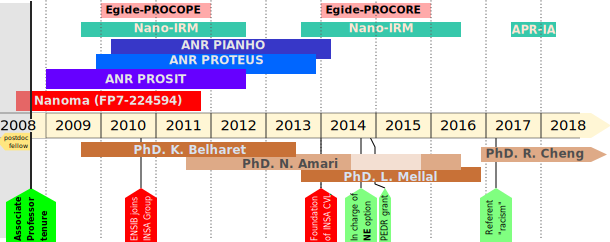
\includegraphics[width=1\linewidth-1ex]{fig/chapI/dfolio_timeline} %
  \caption[Progress of main events and activities.]{Progress of main events and activities (\eg projects and supervisions) since  tenure. 
    For further informations on the different project, and the \PhD supervisions refer to appendices\;\ref{sec:CV:projects} and \ref{sec:CV:supervision} respectively.}\label{fig:timeline}
\end{figure}
%
\begin{figure}[tb]
  \centering
  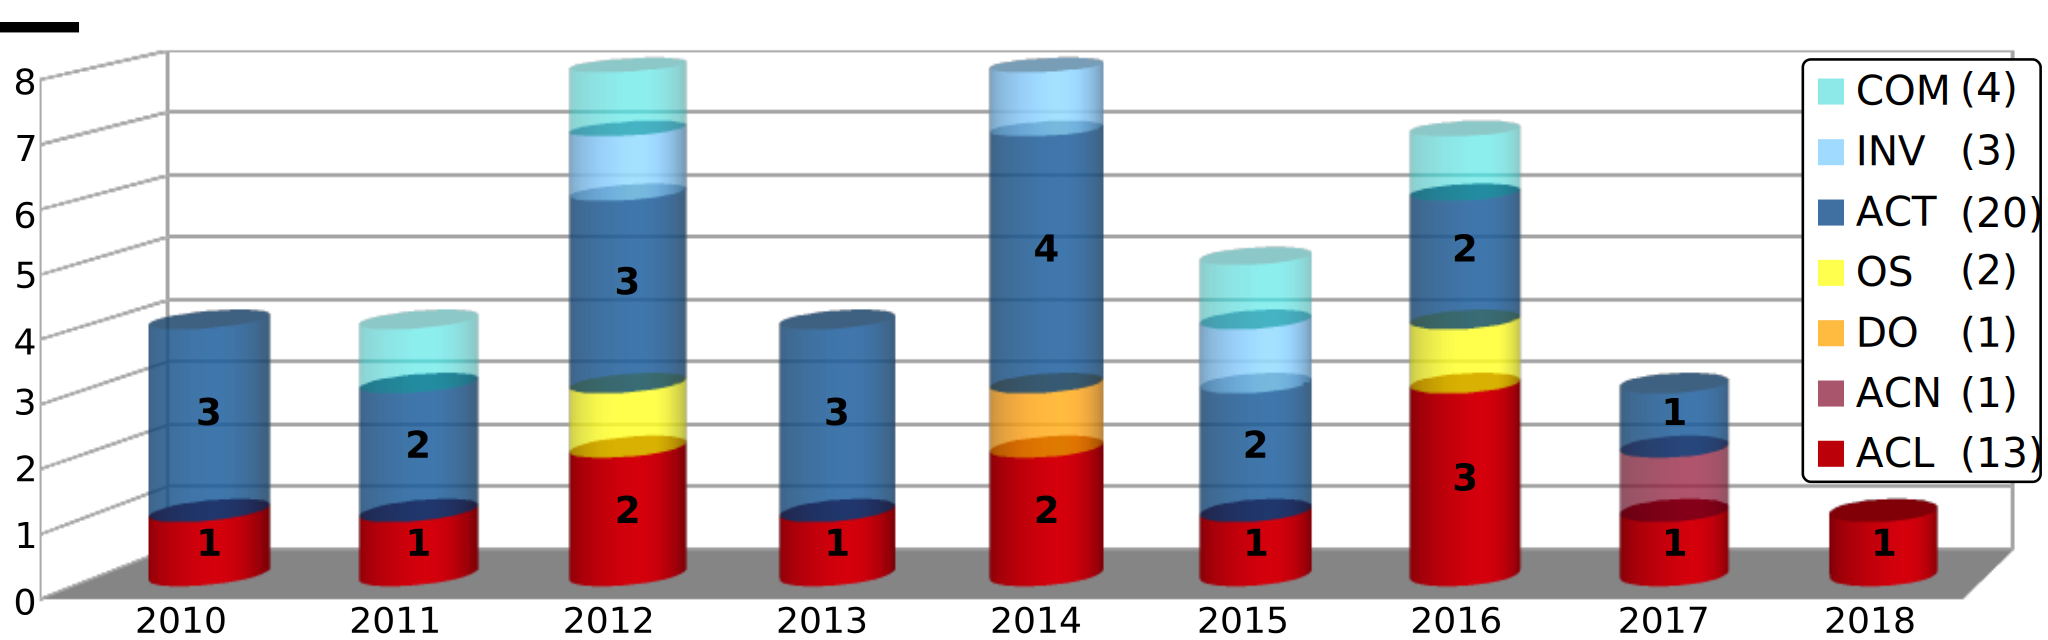
\includegraphics[width=1\linewidth-1ex]{fig/chapI/dfolio_publisAll} %width=1\linewidth-1ex
  \caption[Personal references timeline since tenured as Associate Professor.]{Personal references timeline evolution since tenured as Associate Professor.
    The listed publications follows the nomenclature proposed by the {\EFrench{Haut Conseil de l’évaluation de la recherche et de l’enseignement supérieur} (Hcéres)}\cite{2018_hceres}.
    The detailed list of my publications and the nomenclature are given in appendix\;\RefAnnexeRef. }
  \label{fig:publis}
\end{figure}

Furthermore, I perform my research activities with the \PRISMEshort\footnote{{\acrlong{PRISME}} (PRISME) Laboratory is from University of Orléans  and \INSAshort \CVL (EPRES 4229). \url{http://www.univ-orleans.fr/PRISME}.}  
Laboratory in the Robotics team of the Images, Robotics, Automatic control and Signal (IRAuS) unit.
Since I am an Associate Professor, my research interests mainly deal with the modeling and control for nano and micro-robotics in a biomedical context.
It can be noticed that I had to apply a slight change of my research topics  to address the specificities of the microworld.
Actually, in a first time, my research activities have been mainly related with the European project \acrshort{NANOMA}\footnote{\acrlong{NANOMA} (see also\;\protect\ref{proj:NANOMA})}.
This project consisted to design microrobotic system for targeted drug delivery through the cardiovascular system.
Parallelly, I have also contributed to the development of micromanipulation activities of the laboratory.
Firstly, the micromanipulation has been devoted for intra-cytoplasmic applications\cite{2011_icra_kim,2012_tase_kim}.
Next, this research activities evolved to object micromanipulation to be placed in the focus of a light beam within the \ANRshort project \PIANHOfoot\ref{proj:PIANHO}.
The different projects in which I have been involved are reported in the \autoref{fig:timeline}, and detailed in appendix\;\ref{sec:CV:projects}.
%\smallskip
In addition, I have directly co-supervised the works of 4 \PhD students (with one still on going), with their names also reported in the \autoref{fig:timeline}.
I also  had the opportunity to follow the research works of 5 external \PhD students. 
Further informations about these supervisions are given in the appendix\;\ref{sec:CV:supervision}.

Since tenured in 2008, these various scientific activities have led,  to 43 publications, including\footnote{The bibliography categories follow the nomenclature proposed by the \EFrench{Haut Conseil de l’évaluation de la recherche et de l’enseignement supérieur} (Hcéres)\cite{2018_hceres}.
Hcéres stand for the High Council for Evaluation of Research and Higher Education, and it is an independent administrative authority.  \url{http://www.hceres.fr}} 13 articles (ACL), 1 guest editorial (DO), 2 books chapter (OS) and 20 proceedings (ACT).
\autoref{fig:publis} illustrates the timeline progress of my publishing activities and the detailed list of my publications are given in appendix\;\RefAnnexeRef. 
As of 2018, I had an H-index of 12 based on Google Scholar Citations\footnote{See also my Google Scholar profile: \url{http://scholar.google.com/citations?user=XQVc6JMAAAAJ}}. 

% ---------------------------------------------------------------------------------
% SECTION -------------------------------------------------------------------------
\section{Activities Organization}\label{sec:activities}

\subsection{Research Context}\label{sec:research:context}
\subsection{Scientific Topics}\label{sec:research}

\subsubsection{subsub section}\label{sec:subsubsection}
\paragraph{paragraph}\label{sec:paragraph}
\subparagraph{subparagraph}\label{sec:subparagraph}

% ---------------------------------------------------------------------------------
% SECTION -------------------------------------------------------------------------
\section{Manuscript Overview}\label{sec:org}



\subsection{sub section}\label{sec:subsectionA}
\subsection{sub section}\label{sec:subsectionB}
\subsection{sub section}\label{sec:subsectionC}
\subsection{sub section}\label{sec:subsectionD}




\endinput
%% --------------------------------------------------------------------------------
%% End of file --------------------------------------------------------------------